
\documentclass{beamer}


\usetheme{Warsaw}
\usecolortheme{crane}


\title{Tensor Analysis}
\subtitle{Mathematical Methods in the Physical Sciences}
\author{Steve Mazza}
\institute[Naval Postgraduate School]
{ 
    Naval Postgraduate School \\
    Monterey, CA \\
    
\includegraphics[height=3cm]{images/NPS_logo.jpg}
}
\date {SE3030, Winter/2014 \\ Quantitative Methods of Systems Engineering}
\subject{Quantitative Methods of Systems Engineering}


\begin{document}

\frame{\titlepage}


\frame{{Introduction}
  \begin{columns}[c]
  \column{.6\textwidth}
  \begin{itemize}
    \item Tensors are designated by their size and \emph{order}.
    \item Tensors of order 0 are scalars
    \item Tensors of order 1 are vectors
    \item A second order tensor has $3^2=9$ components
  \end{itemize}
  \column{.5\textwidth}
    \begin{center}
      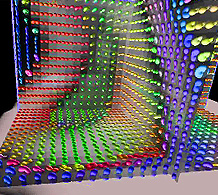
\includegraphics[scale=0.6]{images/tensors.jpg}
    \end{center}
  \end{columns}
}


\frame{{Cartesian Tensors}
  %TODO: Enter reminder. (mazzas) Tue Feb 18 07:28:37 2014
}


\frame{{Tensor Notation and Operations}
  \begin{itemize}
    \item For simplicity, we drop the summation sign and assume summation over any index which appears twice in one term.
    \item Contraction
      \begin{itemize}
        \item Obtained by setting unlike indices equal and summing
        \item Reduces the order by 2
      \end{itemize}
    \item First and second order tensors can be displayed as matrices.
    \item Symmetry
      \begin{itemize}
        \item Symmetric if $T_{ij}=T_{ji}$.
        \item Antisymmetric if $T_{ij}=-T_{ji}$.
        \item Any second order tensor can be written as a sum of a symmetric and antisymmetric tensor.
      \end{itemize}
    \item Combination
      \begin{itemize}
        \item The linear combination of two tensors of order $n$ is a tensor of order $n$.
        \item Addition is not defined for tensors of different order.
      \end{itemize}
    \item Quotient Rule is useful for identifying components of a tensor.
  \end{itemize}
}


\frame{{Inertia Tensor}
  For a rigid body rotating about a fixed axis, we know that the velocity, $\omega$, and momentum, $L$, are related by the equation $L=I\omega$ where $I$ is the moment of inertia.  But if the rotation axis is not fixed, then $I$ must be replaced by a second order tensor with components $I_{jk}$.
}


\frame{{Kronecker Delta and Levi-Civita Symbol}
  \begin{block}{Kronecker Delta}
    \[\delta_{ij} = 1 \text{ if } i=j, 0 \text{ otherwise}\]
  \end{block}
  \begin{block}{Levi-Civita Symbol}
  \begin{align*}
    \epsilon_{ijk} =\ &1 \text{ for an even permutation, } \\
    -&1 \text{ for an odd permutation, and } \\
    &0 \text{ if any indices are repeated.}
  \end{align*}
  \end{block}
}


\frame{{Pseudovectors and Pseudotensors}
  %TODO: Enter reminder. (mazzas) Tue Feb 18 07:33:53 2014
}


\frame{{More About Applications}
  %TODO: Enter reminder. (mazzas) Tue Feb 18 07:33:53 2014
}


\frame{{Curvilinear Coordinates}
  %TODO: Enter reminder. (mazzas) Tue Feb 18 07:33:53 2014
}


\frame{{Vector Operations in Orthogonal Curvilinear Coordinates}
  %TODO: Enter reminder. (mazzas) Tue Feb 18 07:33:53 2014
}


\frame{{Non-Cartesian Tensors}
  %TODO: Enter reminder. (mazzas) Tue Feb 18 07:33:53 2014
}


\frame{{Miscellaneous Problems}
  %TODO: Enter reminder. (mazzas) Tue Feb 18 07:33:53 2014
}


\frame{{Questions?}
	\begin{center}
		
\includegraphics[width=.7\textwidth]{images/fin.png}
	\end{center}
}

\end{document}
